\section{Learning Node Embeddings}
Following \cite{node-emb-latent-space}, we project nodes into a latent space and the geometric relations in that space correspond to those in the original graph.
\begin{marginfigure}
	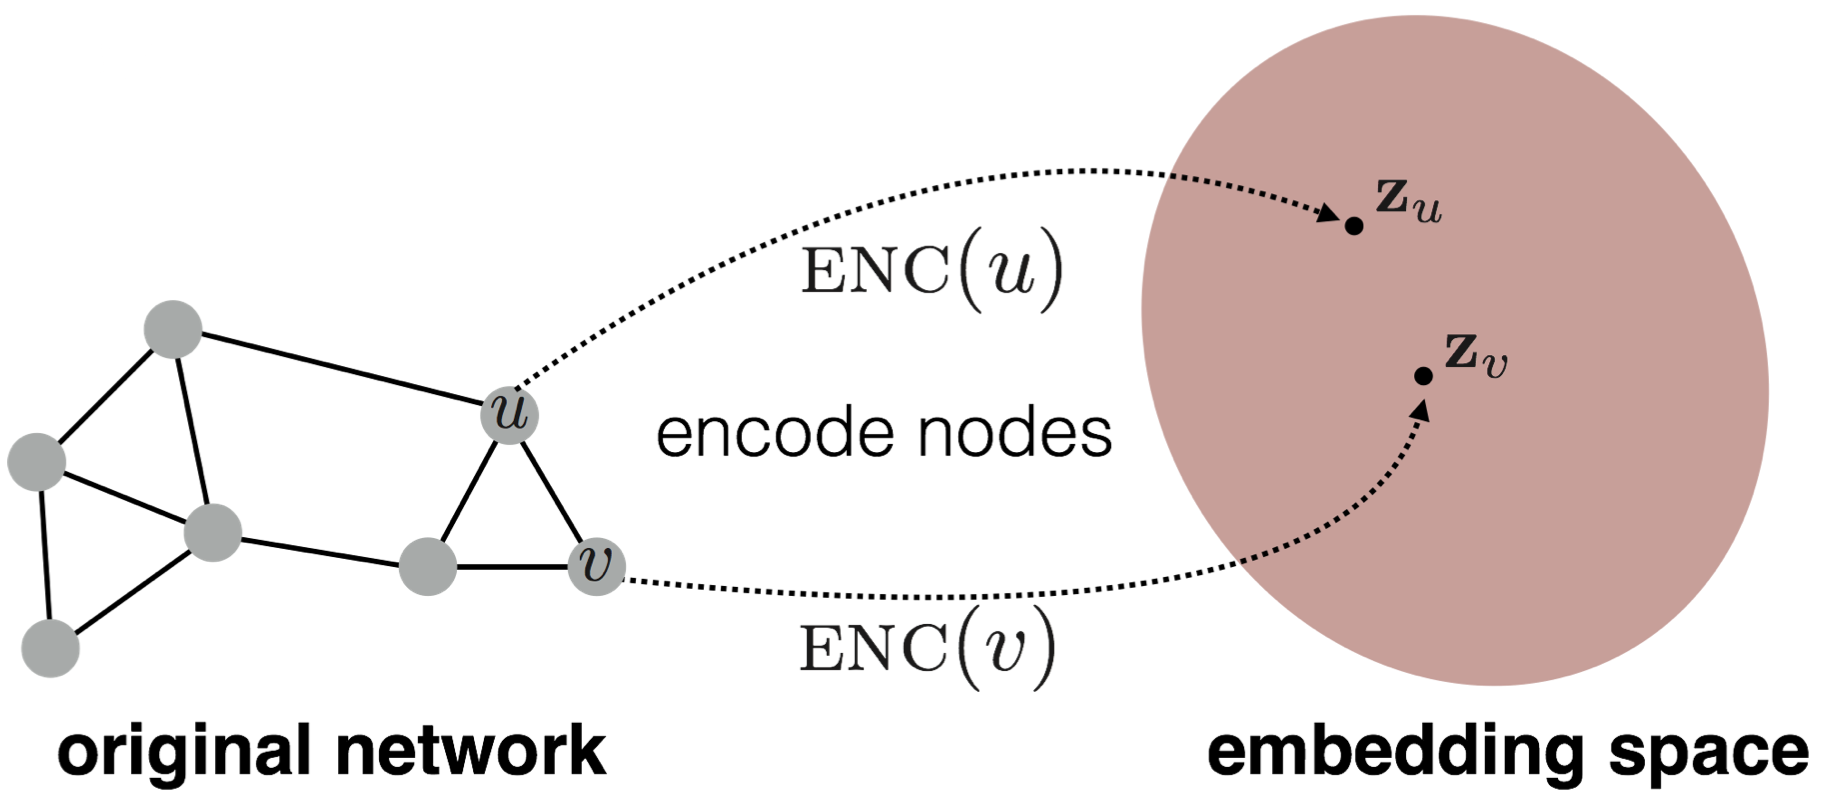
\includegraphics[width=\textwidth]{node-embeddings.png}
	\caption{Node Representation Learning Source: \href{https://snap-stanford.github.io/cs224w-notes/machine-learning-with-networks/node-representation-learning}{Stanford}}
	\label{fig:node-embedding}
\end{marginfigure}
\subsection{Encoder-Decoder Model}
The task is essentially to \textit{encode} each node into a low-dimensional vector, and finally \textit{decode} the embedding and use it to reconstruct information \cite{representation-learning-methods}.
\begin{definition}[Encoder]
The encoder is a function \texttt{ENC}$:V \to \mathbb{R}^d$ which maps nodes $v \in V$ to vector embeddings $\mathbf{z}_v \in \mathbb{R}^d$.. Commonly the approach is a shallow embedding one, and thus the encoder function is an embedding lookup on the node ID, i.e \texttt{ENC}$(v) = \mathbf{Z}[v]$ where $\mathbf{Z} \in \mathbb{R}^{|V| \times d}$ is the embedding matrix.
\end{definition}
\begin{definition}[Decoder]
The decoder reconstructs certain graph statistics from node embeddings generated by the encoder. It is common to use pairwise decoders, i.e \texttt{DEC}$:\mathbb{R}^d \times \mathbb{R}^d \to \mathbb{R}^+$ and they are similarity measures.
\end{definition}
The goal is to minimize reconstruction loss, i.e 
\begin{equation}\label{eq:recon-loss}
\texttt{DEC}(\texttt{ENC}(u), \texttt{ENC}(v)) = \texttt{DEC}(\mathbf{z}_u, \mathbf{z}_v) \approx \mathbf{S}[u, v]
\end{equation}
\marginnote{
	Mean Squared Error loss:
	\begin{equation*}
		MSE(y, \tilde{y}) = \dfrac{1}{n}\sum_{i=1}^n (y_i - \tilde{y}_i)^2
	\end{equation*}
	Cross Entropy loss:
	\begin{equation*}
		CE(y, \tilde{y}) = -\dfrac{1}{n}\sum_{i=1}^n y_i \log(\tilde{y}_i)
	\end{equation*}
}
To achieve the goal above, we minimize an empirical reconstruction loss function
\begin{equation}
\mathcal{L} = \sum_{(u, v) \in \mathcal{D}} \ell(\texttt{DEC}(\mathbf{z}_u, \mathbf{z}_v), \mathbf{S}[u,v])
\end{equation}
\noindent where $\mathcal{D}$ is a subset of node pairs, and $\ell$ is a loss function such as cross-entropy or mean-squared error loss. We look at some common shallow embedding algorithms:
\begin{enumerate}
\item \textbf{Factorization based Encoder-Decoder}\\
The loss function for such approaches can be minimized using factorization algorithms such as SVD.
\begin{enumerate}
\item \textbf{Laplacian Eigenmaps} \cite{laplacian-eigenmaps}: 
	\marginnote{If we construct $\mathbf{S}$ to satisfy properties of $\mathbf{L}$, and $\mathbf{z}_u$ are $d$-dimensional, then the optimal solution for minimizing the loss is given by the $d$ smallest eigenvectors of $\mathbf{L}$ excluding the smallest one, i.e $\mathbf{1}$}
It is an old but influential approach built upon spectral clustering. The decoder is 
\begin{equation}
	\texttt{DEC}(\mathbf{z}_u, \mathbf{z}_v) = ||\mathbf{z}_u - \mathbf{z}_v||_2^2
\end{equation}
and the loss function is
 \begin{equation}
\mathcal{L} = \sum_{(u,v) \in \mathcal{D}} \texttt{DEC}(\mathbf{z}_u, \mathbf{z}_v)\mathbf{S}[u,v]
\end{equation}
\item \textbf{Inner-product methods}: The decoder in these is 
\begin{equation}
\texttt{DEC}(\mathbf{z}_u, \mathbf{z}_v) = \mathbf{z}_u^T\mathbf{z}_v
\end{equation}
and the loss function is
\begin{equation}
\mathcal{L} = \sum_{(u,v) \in \mathcal{D}} ||\texttt{DEC}(\mathbf{z}_u, \mathbf{z}_v) - \mathbf{S}[u,v]||_2^2
\end{equation}

\begin{enumerate}
	\item \textit{Graph Factorization} \cite{graph-factorization}: It uses $\mathbf{S} \triangleq \mathbf{A}$.
	\item \textit{GraRep} \cite{grarep}: It defines $\mathbf{S}$ based on powers of $\mathbf{A}$.
	\item \textit{HOPE} \cite{hope}: It defines $\mathbf{S}$ based on neighborhood overlap measures.
\end{enumerate}
\end{enumerate}
\item \textbf{Random Walk Embeddings} \\
The notion in such embeddings are that two nodes have similar embeddings if they tend to co-occur on short random walks over the graph. We learn embeddings to get
\begin{equation} \label{eq:random-walk-decoder}
\texttt{DEC}(\mathbf{z}_u, \mathbf{z}_v) \triangleq \dfrac{e^{\mathbf{z}_u^T \mathbf{z}_v}}{\sum_{w \in V} e^{\mathbf{z}_u^T \mathbf{z}_w}} \approx p_{G, T}(v|u)
\end{equation}
\marginnote{The notation $\Iintv{x,y}$ denotes the integer interval spanning from $x$ to $y$, i.e $\{x, \cdots y\}$}
where $p_{G,T}(v|u)$ is the probability of reaching node $v$ starting at $u$ on a $T$-length random walk ($T \in \Iintv{2, 10}$). Clearly the decoder is learning an asymmetric stochastic measure. To train the embeddings, the loss function employed is
\begin{equation}
\mathcal{L} = \sum_{(u,v) \in \mathcal{D}} -\log(\texttt{DEC}(\mathbf{z}_u, \mathbf{z}_v))
\end{equation}
	\marginnote{It has been shown in \cite{network-embedding-matrix} that if we define 
	\begin{equation*}
		\mathbf{S}_{DW} = \log\bigg(\dfrac{\sum_{w \in V}d_w}{T} \Big(\sum_{t=1}^T\mathbf{P}^t\Big)\mathbf{D}^{-1}\bigg) - \log (b)
	\end{equation*}
	then, the embeddings $\mathbf{Z}$ by DeepWalk satisfy $\mathbf{Z}^T \mathbf{Z} \approx \mathbf{S}_{DW}$. What is interesting to note that is we can eigendecompose the interior of above equation, and note that DeepWalk is closely related to $\mathbf{L}_{sym}$ and hence spectral clustering, but differ by the fact that influence of eigenvalues is controlled by DeepWalk through $T$.
}
But the issue here is that evaluating the loss function has time complexity $\mathcal{O}(|V||\mathcal{D}|) \sim \mathcal{O}(|V|^2)$.
\begin{enumerate}
	\item \textbf{DeepWalk} \cite{deepwalk}: 
	It employs uniformly random walks to define $p_{G,T}(v|u)$ and employs hierarchical softmax \cite{hierarchical-softmax} to approximate Equation (\ref{eq:random-walk-decoder})
	\item \textbf{node2vec} \cite{node2vec}: It introduces hyperparameters to allow random walk probabilities to interpolate between walks more akin to BFS or DFS. It uses noise contrastive estimation along with negative sampling to rewrite $\mathcal{L}$ as
	\begin{equation}
	\mathcal{L} = \sum_{(u,v)\in\mathcal{D}} -\log(\sigma(\mathbf{z}_u^T\mathbf{z}_v)) - \gamma \mathbb{E}_{v_n \sim P_n(V)}[\log(-\sigma(\mathbf{z}_u^T \mathbf{z_{v_n}}))]
	\end{equation}
	with $\gamma > 0$ and $P_n(V)$ being the uniform distribution. Monte Carlo Sampling is used to calculate the expectation.
	\item \textbf{LINE} \cite{line}: It proposes a first objective
	\begin{equation}
		\texttt{DEC}(\mathbf{z}_u, \mathbf{z}_v) = \sigma(\mathbf{z}_u^T\mathbf{z}_v)
	\end{equation}
\marginnote{
\textbf{KL-Divergence}
\begin{equation*}
	D_{KL}(p \parallel q) = \sum_{i=1}^n p(x_i) \log\bigg(\dfrac{p(x_i)}{q(x_i)}\bigg)
\end{equation*}
}
and $\mathbf{S}[u,v] = A_{uv}$. Along with that, a second objective is the decoder same as DeepWalk, but trained using KL-Divergence to encode 2-hop information (i.e $\mathbf{A}^2$), and it explicitly reconstructs first and second-order neighborhood information.
\end{enumerate}
\end{enumerate}
\subsection{Drawbacks of Shallow Embeddings}
\begin{itemize}
	\item[$\diamond$] Lack of parameter sharing between nodes is a hinder to statistic and computational efficiency. We want embeddings to be independent of $|V|$.
	\item[$\diamond$] They do not leverage node features in \texttt{ENC}.
	\item[$\diamond$] They are transductive, and thus it is difficult to generate embeddings for newer nodes and cannot be used in inductive applications which involve generalization.
\end{itemize}